\documentclass[tikz,border=10pt]{standalone}
\begin{document}
    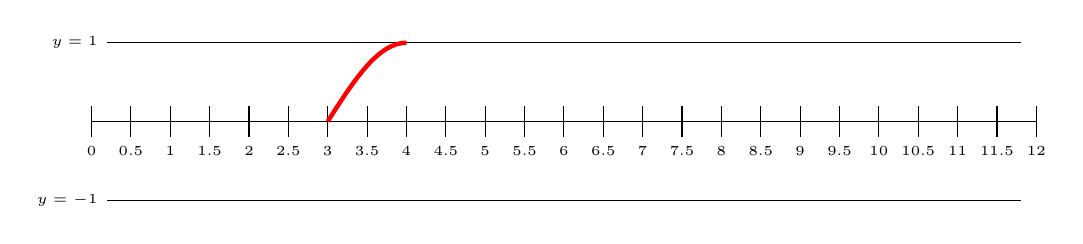
\begin{tikzpicture}
    \draw (0,0) -- (12,0);
    \draw (0.2,1)node[left,font=\tiny] {$y=1$} -- (11.8,1);
    \draw (0.2,-1)node[left,font=\tiny] {$y=-1$} -- (11.8,-1); 
    \foreach \x in {0,0.5,...,12}{
    \draw (\x,-0.2)node [below,font=\tiny,] {\x} -- (\x,0.2) ;
    }
    \draw[ultra thick, red] (3,0) sin (4,1);    %% the real business in this line
    \end{tikzpicture}
\end{document}